\documentclass[10pt, reqno]{article}

\usepackage{amsfonts,latexsym,amsthm,amssymb,amsmath,amscd,euscript,bm}
\usepackage[sc]{mathpazo}
\usepackage[margin = 2cm]{geometry}
\usepackage{enumitem}
\usepackage{hyperref}
\usepackage{slashed}
\usepackage{xcolor}
% sets numbering of enumerate to a, b, c, ...
\renewcommand{\theenumi}{\alph{enumi}}

% Theorems, propositions, etc.
\newtheorem{theorem}{Theorem}
\newtheorem{proposition}[theorem]{Proposition}
\newtheorem{lemma}[theorem]{Lemma}
\newtheorem{corollary}[theorem]{Corollary}

\theoremstyle{definition}
\newtheorem{definition}[theorem]{Definition}
\newtheorem*{claim}{Claim}

\theoremstyle{remark}
\newtheorem*{remark}{Remark}
\newtheorem*{notation}{Notation}

\usepackage{thmtools}
\usepackage[framemethod=TikZ]{mdframed}
	\mdfdefinestyle{mdrecbox}
		{%
			linewidth=0.5pt,
			skipabove=12pt,
			frametitleaboveskip=5pt,
			frametitlebelowskip=0pt,
			skipbelow=2pt,
			frametitlefont=\bfseries,
			innertopmargin=4pt,
			innerbottommargin=8pt,
			nobreak=true,
		}
	\declaretheoremstyle
		[
			headfont=\bfseries,
			mdframed={style=mdrecbox},
			headpunct={\\[3pt]},
			postheadspace={0pt},
		]
		{thmrecbox}
	\declaretheorem[style=thmrecbox,name=Example, numberlike=theorem]{examplebox}

\newenvironment{example}
	{
	\begin{examplebox} 
	\leavevmode
	\begin{enumerate}}
	{	\end{enumerate} 
	\end{examplebox}
	}


% Math blackboard font
\newcommand{\nc}{\newcommand}
\nc{\on}[1]{\operatorname{#1}}

\nc{\R}{\mathbb R}
\nc{\C}{\mathbb C}
\nc{\Q}{\mathbb Q}
\nc{\Z}{\mathbb Z}
\nc{\N}{\mathbb N}
\nc{\HH}{\mathbb H}
\nc{\DD}{\mathbb D}
\nc{\TT}{\mathbb T}

\nc{\cT}{\mathcal T}
\nc{\cP}{\mathcal P}
\nc{\cM}{\mathcal M}
\nc{\cC}{\mathcal C}
\nc{\cB}{\mathcal B}
\nc{\cG}{\mathcal G}
\nc{\cA}{\mathcal A}
\nc{\cS}{\mathcal S}
\nc{\cF}{\mathcal F}
\nc{\cL}{\mathcal L}
\nc{\cR}{\mathcal R}

\nc{\diam}{\operatorname{diam}}
\nc{\del}{\partial}
\nc{\inter}{\mathrm{o}}
\nc{\close}[1]{\overline{#1}}
\nc{\supp}{\operatorname{supp}}
\nc{\loc}{\text{loc}}
\nc{\length}{\operatorname{length}}
\nc{\Ric}{\operatorname{Ric}}
% Why the f*** would you ever use \epsilon
\renewcommand{\epsilon}{\varepsilon}
\renewcommand{\emph}{\textsc}

\let\vec\mathbf


% Title: change problem set number as needed
\title
{
	\emph{Non-linear wave equations and general relativity}
} 

\author{Jason Zhao}
\date{\emph{Fall 2021}}

\begin{document}

\maketitle

\begin{abstract}
	Notes on the seminar organised by Sung-Jin Oh introducing the vector field method and its applications to non-linear wave equations and general relativity. 
\end{abstract}

\tableofcontents

\section{Introduction to the vector field method}
Consider the linear wave equation, 
\begin{align}
	\Box \phi  					&= f, \notag \\
	\phi_{|t = 0}				&= g, \label{eq:linearwave}\\
	\partial_t \phi_{|t = 0}	&= h.\notag
\end{align}
This will be the prototype for the study of other equations such as the Einstein equation. One natural question is to ask about the pointwise behavior of the solution as time moves forward $t\to \infty$. In the homogeneous case taking $f = 0$ and $g = 0$ in four-dimensional space-time, $\R_t \times \R^3_x$, we simply consider the fundamental solution as given by Kirchhoff's formula, 
	\[ \phi(t, x) = \frac{1}{4\pi t} \int_{\partial B_t (x)} h dS(y). \]
Assuming $h \in C_c^\infty (\R^3_x)$ furnishes the pointwise bound
	\[ |\phi(t, x)| \lesssim \frac{1}{1 + t} \]	
uniformly in space. While this estimate is good in that we can easily compute the implicit constant, the method of analyzing the fundamental solution is not robust, particularly when considering equations with non-linearity or other differential operators. This motivates the use of the vector field method \'a la Klainerman \cite{Klainerman1985}, based on energy estimates and commuting vector fields which we obtain from symmetries with $\Box$. 

\subsection{Energy estimates}
We begin with the following integration by parts formula which gives the change in the Dirichlet energy of our solution from $t = t_0$ and $t = t_1$;

\begin{theorem}[Conservation of energy]
	Let $t_0 < t_1$ and $\phi$ be a solution to the $(d + 1)$-dimensional linear homogeneous wave equation (\ref{eq:linearwave}) with smooth compactly supported initial data. Then 
		\[ \int_{t = t_1} \frac12 |\nabla_{t, x} \phi|^2 \, dx = \int_{t = t_0} \frac12 |\nabla_{t, x} \phi|^2 \, dx - \int_{t_0}^{t_1} \int_{\R^d} f \, \partial_t \phi \, dx \, dt.  \] \label{thm:conserve}
\end{theorem}

\begin{proof}
	Introducing a factor of $\partial_t \phi$ to both sides of the wave equation, we can write
		\begin{align*}
		f \partial_t \phi 
			= \Box \phi \, \partial_t \phi  
			&= \left(- \partial_t^2 \phi + \sum_{j = 1}^n \partial_j^2 \phi\right) \partial_t \phi \\
			&= \partial_t \left( -\frac12 (\partial_t \phi)^2 \right) + \sum_{j = 1}^n \partial_j \left( \partial_j \phi \, \partial_t \phi \right) - \partial_j \phi \, \partial_t \partial_j \phi\\
			&= \partial_t \left( -\frac12 (\partial_t \phi)^2 - \frac12 \sum_{j = 1}^n (\partial_j \phi)^2 \right) + \nabla_x \cdot (\partial_t \phi \, \nabla_x \phi).
	\end{align*}
	We integrate both sides over the region $(t_0, t_1) \times \R^d$. By the divergence theorem, the second term on the right vanishes, so rearranging furnishes the identity. 
\end{proof}

\begin{remark}
	The identity used in the proof of conservation of energy is known as the \emph{multiplier identity for $\partial_t$}.
\end{remark}


\begin{corollary}[Energy estimate]
	Let $t_0 < t_1$ and $\phi$ be a solution to the $(d + 1)$-dimensional linear homogeneous wave equation (\ref{eq:linearwave}) with smooth compactly supported initial data. Then
		\[ \sup_{t \in [t_0, t_1]}||\nabla_{t, x} \phi||_{L^2_x} (t) \lesssim ||\nabla_{t, x} \phi||_{L^2_x} (t_0)+ \int_{t_0}^{t_1} ||f||_{L^2_x} (t) \, dt.  \]
\label{cor:energyest1}
\end{corollary}

\begin{proof}
	Applying the triangle inequality to the conservation of energy identity,
		\[\frac12 \sup_{t \in [t_0, t_1]} ||\nabla_{t, x} \phi\|_{L^2_x}^2 (t) \leq \frac12 ||\nabla_{t, x} \phi ||_{L^2_x}^2 (t_0) + \int_{t_0}^{t_1} ||f \, \partial_t \phi ||_{L^1_x} (t) \, dt. \]
	It remains to control the regularity of the second term on the right. Fix $\epsilon > 0$ to be chosen later, then applying Holder's inequality, the inequality of arithmetic and geometric means gives
		\[ \int_{t_0}^{t_1} ||f \, \partial_t \phi ||_{L^1_x} (t) \, dt \leq \int_{t_0}^{t_1} ||f||_{L_x^2} (t) \, ||\partial_t \phi||_{L_x^2} (t) \, dt \leq \frac12\int_{t_0}^{t_1} \left( \frac{1}{\epsilon} ||f||_{L^2_x}^2 (t) + \epsilon ||\partial_t \phi||_{L^2_x}^2 (t) \right) \, dt \]	
	Choosing $\epsilon \ll 1$, the second term on the right is absorbed into $||\nabla_{t, x} \phi||_{L^2_x}$, so we conclude the energy estimate.
\end{proof}

To obtain a quantitative pointwise bound on $\nabla_{t, x} \phi$, we argue by Sobolev embedding. Note that $\partial_j$ commutes with the wave operator $\Box$, so the derivatives of $\phi$ are also solutions to the wave equation, satisfying $\Box (\partial^{\alpha} \phi) = \partial^\alpha f$ for any multi-index $\alpha \in \N^d$. The corresponding energy estimates are
	\[ ||\partial^\alpha \nabla_{t, x} \phi||_{L^\infty_t L_x^2 (t_0, t_1)} \lesssim_\alpha ||\partial^{\alpha} \nabla_{t, x} \phi ||_{L^2_x} (t_0) + ||\partial^\alpha f||_{L^1_t L^2_x (t_0, t_1)}.  \]
Summing over the multi-indices $|\alpha|\leq k$, we obtain the corresponding estimates for the Sobolev norms $H^k_x$. It follows from Sobolev embedding that
	\[ ||\nabla_{t, x} \phi||_{L^\infty_t L^\infty_x (t_0, t_1)}  \lesssim ||\nabla_{t, x} \phi||_{H^k_x} (t_0) + ||f||_{L^1_t H^k_x (t_0, t_1)} \]
for any $k > d/2$. In particular, taking $t_0 = 0$ and $f = 0$, we have pointwise control over $\nabla_{t, x} \phi$ by the regularity of initial data. Note that we derived pointwise boundedness using only vector fields $\partial^\alpha$ corresponding to symmetries of Euclidean space $\R^d_x$. To derive pointwise decay, i.e. a \textit{dispersive estimate}, we need to exploit the symmetries of Minkowski space-time $\R_t \times \R^d_x$, namely the vector fields $\sum_\alpha x^\alpha \partial^\alpha$ which commute with $\Box$.
	
\subsection{Commuting vector fields and symmetry}

How exactly do we go about finding commuting vector fields? These correspond exactly to symmetries in our partial differential operator, which in turn correspond to symmetries in space-time. More explicitly, recall that the wave operator is exactly the Laplace-Beltrami operator corresponding to Minkowski space-time $(\R_t \times \R^d_x, M)$, where $M$ is the quadratic form with matrix representation
	\[ 
		M 
		=
		\begin{pmatrix}
			-1	& 		& 			&0 \\
				& 1	&			&  \\
				&		&\ddots 	&  \\
			0	&		& 			&1
		\end{pmatrix}.
	\]
Denoting $x^0 = t$, it follows that 
	\[ \Box = -\partial_t^2 + \sum_{j = 1}^d \partial_j^2 = \sum_{j, k = 0}^d M^{j, k} \partial_j \partial_k. \]	
Then the affine maps $T: \R_t \times \R^d_x \to \R_t \times \R^d_x$ preserving the quadratic form $M$, i.e. $T^t M T = M$, are exactly the affine maps preserving the wave operator, i.e. $\Box (\phi \circ T) = (\Box \phi) \circ T$. These maps give rise to the \emph{Poincare group}, which is generated by the following:
\begin{itemize}
	\item Spatial translations; for example, translation in the $x^1$ coordinate by $s \in \R$:
				\[ T\begin{pmatrix} t \\ x^1 \\ x^2\\ \vdots \\ x^d \end{pmatrix} =  \begin{pmatrix} t \\ x^1 + s \\ x^2 \\ \vdots  \\ x^d \end{pmatrix}.\]
			Infinitesimal translation in the $x^k$-spatial coordinate corresponds to the vector field $\partial_k$. 	
	
	\item Spatial rotations; for example, rotation in the $(x^1, x^2)$-plane by $\theta \in S^1$:
				\[
					T \begin{pmatrix} t \\ x^1 \\ x^2 \\ x^3 \\ \vdots \\ x^d \end{pmatrix}
					=
					\begin{pmatrix} t \\ x^1 \cos \theta  -x^2 \sin \theta  \\ x^1 \sin \theta  +  x^2 \cos \theta  \\  x^3 \\ \vdots \\ x^d \end{pmatrix}.
				\]
			Infinitesimal rotation in the $(x^j, x^k)$-plane corresponds to the vector field $\Omega_{j, k} := x^j \partial_k - x^k \partial_j$. 
	
	\item Lorentz boosts; these transformations are essentially rotations in the time coordinate. Let $v \in \R^d$ with $|v| < 1$, then an example of a boost is
				\[
					T
					\begin{pmatrix} t \\ x^1 \\ x^2 \\ \vdots \\ x^d \end{pmatrix}
					 = \begin{pmatrix} \frac{1}{\sqrt{1 - |v|^2}} (t - v x^1) \\  \frac{1}{\sqrt{1 - |v|^2}} (x^1 - v t) \\ x^2 \\ \vdots \\ x^d \end{pmatrix}
				 \]
			The infinitesimal Lorentz boost in the $x^j$-spatial coordinate corresponds to the vector field $H_j = t \partial_j + x^j \partial_t$. 	 
\end{itemize}
Adding scaling to the Poincare group gives rise to the \emph{Lorentz group}:
\begin{itemize}
	\item Spatial scaling; for example, scaling by $\lambda > 0$ of space is given by 
				\[
					T
					\begin{pmatrix}
						t \\ x^1 \\ \vdots \\ x^d
					\end{pmatrix}
					=
					\begin{pmatrix}
						t \\ \lambda x^1\\ \vdots \\ \lambda x^d
					\end{pmatrix}
				\]
			Infinitesimal scaling in space corresponds to the vector field $S = t \partial_t + \sum_j x^j \partial_j$. 		 
\end{itemize}
The first three vector fields commute with the wave operator, that is, $[\partial_k, \Box] = [\Omega_{j, k}, \Box] = [H_j, \Box] = 0$. While scaling is not a full symmetry, it is a conformal symmetry with commutator $[S, \Box] = -2 \Box$. Moreover, the commutator vanishes on solutions to the homogeneous wave equation, i.e. if $\Box \phi = 0$ then $\Box (S \phi) = S(\Box \phi) = 0$. 

Labeling the vector fields $Z_1, \dots, Z_N$ and using the usual multi-index notation $Z^\alpha = Z_1^{\alpha_1} \dots Z_N^{\alpha_N}$, we can extend the energy estimate to $Z^\alpha \phi$;
\begin{theorem}[Energy estimate for $Z^\alpha \phi$]
	Let $\phi$ be a solution to the $(d + 1)$-dimensional linear homogeneous wave equation (\ref{eq:linearwave}) with smooth compactly supported initial data, and suppose $t_0 < t_1$. Then 
		\[ \sum_{|\alpha| \leq k} || \nabla_{t, x} Z^\alpha \phi||_{L^\infty_t L^2_x (t_0, t_1)} \lesssim \sum_{|\alpha| \leq k}|| \nabla_{t, x} Z^\alpha \phi ||_{L^2_x} (t_0). \] \label{thm:energycom}
\end{theorem}
If we want to obtain pointwise bounds on the gradient, following our previous energy method approach it becomes apparent that we need Sobolev-type embedding inequalities with respect to the commuting vector fields.


\subsection{The Klainerman-Sobolev inequality}

To prove the Klainerman-Sobolev inequality, we need to control the usual derivatives $\partial$ pointwise by the commuting vector fields $Z$ with some additional weights. For example, we will need the following lemma:

\begin{lemma}	
	For $(t, x) \in (0, \infty) \times \R^d$ and $k \in \N$ the following inequality holds
		\[ \sum_{|\alpha| = k} |\partial^\alpha \psi (x, t)| \lesssim_{d, k} \frac{1}{|t - r|^k} \sum_{|\alpha| \leq k} |Z^\alpha \phi (t, x)| \]
	uniformly for $\phi \in C^k (\R_t \times \R_x^d)$. \label{lem:kslem1}	
\end{lemma}

\begin{proof}
	Consider the identities
		\begin{align*}
			\partial_j 
				&= \frac{1}{t^2 - |x|^2} \left( t H_j - x^j S - \sum_{k = 1}^d x^k \Omega_{j, k} \right) = \frac{1}{t - |x|} \left( \frac{t}{t + |x|} H_j - \frac{x^j}{t + |x|} S -\sum_{k = 1}^d\frac{x^k}{t + |x|} \Omega_{j, k} \right) 
		\end{align*}
	and
		\begin{align*}			
			\partial_t
				&= \frac{1}{t^2 - |x|^2} \left( t S - \sum_{k = 1}^d x^k H_k \right) = \frac{1}{t - |x|} \left( \frac{t}{t + |x|} S - \sum_{k = 1}^d \frac{x^k}{t + |x|} H_k \right)
		\end{align*}	
	Applying the identities iteratively furnishes the lemma. 
\end{proof}

\begin{lemma}[Sobolev embedding on cubes]
	Let $Q \subseteq \R^d_x$ be a cube with side lengths $l := (l_1, \dots, l_d)$. Then 
		\[ ||\psi||_{L^\infty_x (Q)} \lesssim \frac{1}{(l_1\cdots l_d)^\frac12} \sum_{|\alpha| \leq \frac{d + 2}{2}} l^\alpha ||\partial^\alpha \psi||_{L^2_x (Q)}. \]\label{lem:kslem2}	
\end{lemma}

\begin{proof}
	The case $l_1 = \dots = l_d = 1$ follows from the usual Sobolev embedding inequality,
		\[ ||\psi||_{L^\infty_x (Q)} \lesssim \sum_{|\alpha| \leq \lfloor\frac{d + 2}{2} \rfloor} ||\partial^\alpha \psi||_{L^2_x}. \]
	The general case follows from applying the inequality above to the rescaled function
		\[ \psi_l (x) := \psi(l_1 x^1, \dots, l_d x^d). \]
\end{proof}

We want to choose cubes with side lengths comparable to the desired weights. The pointwise bound on $\partial^\alpha \psi$ should therefore cancel out the term $l^\alpha$. Decomposing $\R_t \times \R^d_x$ into three different regions, we choose cubes appropriately on each region and apply the previous lemmas to prove the Klainerman-Sobolev inequality:
\begin{theorem}[Klainerman-Sobolev inequality]
	The following inequality holds uniformly for all $\phi \in H_x^{\lfloor \frac{d + 2}{2} \rfloor} (\R_t \times \R^d_x)$ and $(t, x) \in (0, \infty) \times \R^d_x$, 
		\[ |\phi(t, x)| \lesssim_d \frac{1}{(1 + t + r)^{\frac{d - 1}{2}} (1 + |t - r|)^{\frac12}} \sum_{|\alpha| \leq \lfloor \frac{d + 2}{2}\rfloor} ||Z^\alpha \phi||_{L^2_x} (t). \]
\end{theorem}		

\begin{proof}
	This result in the region $t + r \leq 1$ follows directly from the usual Sobolev embedding inequality and the observation that
		\[ (1 + t  +r)^{\frac{d - 1}{2}} (1 + |t - r|)^\frac12 \sim 1, \]
	in this region. Therefore for the remainder of the proof we assume $t + r > 1$. Consider the region $r \leq t/2$; the proof of the result in the region $r \geq 2t$ is symmetric. Define the cube	
		\[ Q =  \left(x^1 - \frac{|t - r|}{100}, x^1 + \frac{|
t - r|}{100}\right) \times \dots \times  \left(x^d - \frac{|t - r|}{100}, x^d + \frac{|
t - r|}{32}\right). \]
	Observe that if $y \in Q$, then $|y| \leq 3t/4$ and moreover $t - |y| \sim t - r$, so by Lemma \ref{lem:kslem1} we have
		\[ \sum_{|\alpha| = k}||\partial^\alpha \phi ||_{L^2_x (Q)} \lesssim \frac{1}{|t - r|^k} \sum_{|\alpha| \leq k} ||Z^\alpha \phi ||_{L^2_x}. \]
	Lemma \ref{lem:kslem2} and the inequality above furnish the result, 
		\[ |\phi (t, x)| \lesssim \frac{1}{|t - r|^{\frac{d}{2}}} \sum_{|\alpha| \leq \lfloor \frac{d + 2}{2} \rfloor} |t - r|^{|\alpha|} ||\partial^\alpha \phi||_{L^2_x (Q)} \lesssim  \frac{1}{|t - r|^{\frac{d}{2}}} \sum_{|\alpha| \leq \lfloor \frac{d + 2}{2} \rfloor} ||Z^\alpha \phi||_{L^2_x}, \]
	since $t - r \sim t + r$ in this region. 		
	
	It remains to show the result in the region $t/2 \leq r \leq 2t$. Rotating the domain, we can assume without loss of generality that $x = (r, 0, \dots, 0)$. Consider the coordinate system 
		\[ (s, y^2, \dots, y^d) := (r, x^2, \dots, x^d). \]
	The tangent vectors in this coordinate system at $x$ are
		\[ \partial_{y^j} = \partial_{x^j} - \frac{x^j}{x^1} \partial_{x^1} = \frac{1}{r} \Omega_{1, j}, \qquad \partial_s = \sum_{j = 1}^d \frac{x^j}{r} \partial_{x^j} = \partial_{x^1}. \]
	In place of Lemma \ref{lem:kslem1}, we instead use the estimates $\partial_{y^j} \sim t^{-1} \Omega_{1, j}$ and $ \partial_s \sim \partial_{x^1}$. Consider the cube
		\[ Q = \left( r - \frac{1 + |t - r|}{100}, r + \frac{1 + |t - r|}{100} \right) \times \left(-\frac{t}{100}, \frac{t}{100} \right) \times \dots \times \left( -\frac{t}{100}, \frac{t}{100} \right) \]	
	in the $(s, y)$-coordinate system, corresponding to a ``curved'' cube in our usual $x$-coordinate system. Similar to the previous case, $y \in Q$ implies that $t/4 \leq |y| \leq 4t$ and moreover $|y| \sim r \sim t \sim 1 + t + r$. Thus by Lemma \ref{lem:kslem2} and our estimates on the tangent vectors in the coordinate system, we obtain
		\[ |\phi(t, x)| \lesssim \frac{1}{(1 + |t - r|)^\frac12 t^{\frac{d - 1}{2}}} \sum_{|\alpha| \leq \lfloor\frac{d + 2}{2}\rfloor} (1 + |t - r|)^{\alpha_s} t^{|\alpha| - \alpha_s} ||\partial_{s, y}^\alpha \phi ||_{L^2_{s, y} (Q)} \lesssim \frac{1}{(1 + |t - r|)^\frac12 t^{\frac{d - 1}{2}}} \sum_{|\alpha| \leq \lfloor\frac{d + 2}{2}\rfloor} ||Z^\alpha \phi||_{L^2_x}. \]
	Since $t \sim 1 + t + r$ in this region, we conclude the result.  	
\end{proof}

Applying the Klainerman-Sobolev inequality and our energy estimates for the commuting vector fields in Theorem \ref{thm:energycom}, we obtain the promised dispersive estimate for the derivative of a solution to the wave equation;

\begin{corollary}
	Let $\phi$ be a solution to the $(d + 1)$-dimensional linear homogeneous wave equation (\ref{eq:linearwave}) with smooth compactly supported initial data. Then
		\[ |\nabla_{t, x} \phi (t, x)| \lesssim \frac{1}{(1 + t)^{\frac{d - 1}{2}}} \sum_{|\alpha| \leq \lfloor \frac{d + 2}{2} \rfloor} ||Z^{\alpha} \nabla_{t, x} \phi ||_{L^2_x} (0).  \] \label{cor:totaldisp}
\end{corollary}

\begin{corollary}
	Let $\phi$ be a solution to the $(d + 1)$-dimensional linear homogeneous wave equation (\ref{eq:linearwave}) with smooth initial data supported in $B(0, R) \subseteq \R^n$. Then
		\[ |\phi (t, x)| \lesssim_{d, R}  \frac{(1 + |t - r|)^{\frac12}}{(1 + t + r)^{\frac{d - 1}{2}} }\sum_{|\alpha| \leq \lfloor \frac{d + 2}{2} \rfloor} ||\partial Z^\alpha \phi||_{L^2_x} (0). \] \label{cor:goodlemma}
\end{corollary}

\subsection{Application to wave equation with quadratic non-linearity}

In this section we aim to illustrate the robustness of the vector field method by deriving an analogous dispersive estimate for the wave equation with a quadratic non-linearity, namely 
	\begin{equation}
		\Box \phi = \partial \phi \partial \phi 	\label{eq:wavequad}
	\end{equation}	
on five-dimensional space-time $\R_t \times \R^4_x$. 

\begin{proposition}[Local energy estimate]
	Let $\phi$ be a solution to (\ref{eq:wavequad}) on $\R_t \times \R^4_x$ with smooth compactly supported initial data. Then for $k \geq 3$ and $T \ll 1$, 
		\[ ||\nabla_{t, x} \phi||_{L^\infty_t H^k_x (0, T)} \lesssim || \nabla_{t, x} \phi ||_{H^k_x} (0).  \]	
\end{proposition}

\begin{proof}
	We prove the case $k = 3$ for concreteness, the general case is similar. The product rule and $[\Box, \partial] = 0$ furnish the identity
		\[ \Box \partial^3 \phi = \partial^3 \Box \phi = \partial^3 (\partial \phi \partial \phi) = 2 \partial( \partial \phi \partial^3 \phi +  \partial^2 \phi \partial^2 \phi) = 2 \partial^4 \phi \partial \phi +  6 \partial^3 \phi \partial^2 \phi. \]
	By Corollary \ref{cor:energyest1}, the energy estimate for the linear wave equation, we have
		\[ ||\partial^3 \nabla_{t, x} \phi ||_{L^\infty_t L^2_x (0, T)} \lesssim ||\partial^3 \nabla_{t, x} \phi||_{L^2_x} (0) + ||\partial^4 \phi \partial \phi||_{L^1_t L^2_x (0, T)} + ||\partial^3 \phi \partial^2 \phi||_{L^1_t L^2_x (0, T)}.  \]
	We want to control the last two terms on the right. By definition, $||\partial^4 \phi||_{L^\infty_t L^2_x (0, T)} \lesssim ||\nabla_{t, x} \phi||_{L^\infty_t H^3_x (0, T)}$ and, by Sobolev embedding in $\R^4_x$, $||\partial \phi||_{L^\infty_t L^\infty_x (0, T)} \lesssim ||\nabla_{t, x} \phi||_{L^\infty_t H^3_x (0, T)}$, so the second term on the right is controlled by
		\begin{align*}
			||\partial^4 \phi \partial \phi||_{L^1_t L^2_x (0, T)} \lesssim ||\nabla_{t, x} \phi||_{L^\infty_t H^3_x (0, T)} ||\partial^4 \phi||_{L^1_t L^2_x (0, T)} \lesssim T ||\nabla_{t, x} \phi||_{L^\infty_t H^3_x (0, T)}^2.
		\end{align*}
	The third term is similarly controlled by an interpolation argument, 
		\[ ||\partial^3 \phi \partial^2 \phi||_{L^1_t L^2_x (0, T)} \lesssim T ||\nabla_{t, x} \phi||_{L^\infty_t H^3_x (0, T)}^2. \]
	Collecting the inequalities, we obtain
		\[ ||\nabla_{t, x} \phi||_{L^\infty_t H^3_x (0, T)} \leq C ||\nabla_{t, x} \phi||_{H^3_x} (0) + C T || \nabla_{t, x} \phi||_{L^\infty_t H^3_x (0, T)}^2 \]
	for some implicit constant $C > 0$ depending only on $k = 3$. We conclude the result by a bootstrap argument; let $B \geq 2(C + 1)$ and suppose $T \geq 0$ such that 
		\[ ||\nabla_{t, x} \phi||_{L^\infty_t H^3_x (0, T)} \leq B ||\nabla_{t, x} \phi||_{H^3_x} (0). \]
	The result clearly holds for $T = 0$ by choice of $B \geq 1$, so the base case of our continuous induction on time is satisfied. We aim to prove a stronger bound than the one assumed.	The previous two inequalities imply
		\[ ||\nabla_{t, x} \phi||_{L^\infty_t H^3_x (0, T)} \leq C ||\nabla_{t, x} \phi||_{H^3_x} (0) + C T B^2 ||\nabla_{t, x} \phi||_{H^3_x} (0)^2, \]
	so it suffices to show
		\[ C ||\nabla_{t, x} \phi||_{H^3_x} (0) + C T B^2 ||\nabla_{t, x} \phi||_{H^3_x} (0)^2\leq \frac12 B||\nabla_{t, x} \phi||_{H^3_x} (0)\]
	to complete the argument. Rearranging, it is equivalent to show
		\[ CTB^2||\nabla_{t, x} \phi||_{H^3_x} (0) \leq \frac12 B - C.\]	
	Choosing $T \ll 1$, depending only on initial data, furnishes the inequality above, and completes the proof. 	
\end{proof}

It is apparent from the proof of local existence that the time interval of existence grows for smaller initial data. This motivates the use of the vector field method to recover global existence given small initial data. The key insight is that the commuting vector fields preserve the structure of the non-linearity. Indeed, we compute
	\[ \Box Z \phi + [Z, \Box] \phi = Z \Box \phi = Z (\partial \phi \partial \phi) = 2 \partial Z \phi \partial \phi + 2\partial \phi \Box[Z, \partial] \phi.\]
Since $[Z, \Box] = 0$ or $-2\Box$, and $[Z, \partial] = 0$ or $\partial$, 
	\[ \sum_{|\alpha| \leq k} \Box Z^\alpha \phi \sim \sum_{|\beta + \gamma| \leq k} \partial Z^{\beta} \phi \partial Z^{\gamma} \phi  \]
modulo constant coefficients on the right-hand side. 

\begin{theorem}[Global small-data energy estimate]
	Let $\phi$ be a solution to (\ref{eq:wavequad}) on $\R_t \times \R^4_x$ with smooth compactly supported initial data. There exists $\epsilon > 0$ such that if 
		\[ \sum_{|\alpha| \leq 6} ||\nabla_{t, x} Z^\alpha \phi||_{L^2_x} (0) \leq \epsilon \]
	then
		\[ \sum_{|\alpha| \leq 6} ||\nabla_{t, x} Z^\alpha \phi||_{L^2} (t) \lesssim \sum_{|\alpha| \leq 6} ||\nabla_{t, x} Z^{\alpha} \phi||_{L^2} (0). \]	\label{thm:nonlin2}
\end{theorem}

\begin{proof}
	It follows from our earlier discussion that
		\[ \sum_{|\alpha| \leq 6} \Box Z^\alpha \phi \sim \sum_{|\beta + \gamma| \leq 6} \partial Z^{\beta} \phi \partial Z^{\gamma} \phi  .\]
	Either $|\beta| \leq 3$ or $|\gamma| \leq 3$, so we can write
		\[ \left| \sum_{|\beta + \gamma| \leq 6} \partial Z^{\beta} \phi \partial Z^{\gamma} \phi  \right| \leq \left( \sum_{|\alpha| \leq 3} |\partial Z^\alpha \phi| \right)\left( \sum_{|\alpha| \leq 6} |\partial Z^\alpha \phi| \right).\]
	We place the sum up to order three terms in $L^\infty_x$ and apply the Klainerman-Sobolev inequality, while we leave the sum up to order six terms in $L^2_x$,
		\[ \left| \left| \left( \sum_{|\alpha| \leq 3} |\partial Z^\alpha \phi| \right)\left( \sum_{|\alpha| \leq 6} |\partial Z^\alpha \phi| \right) \right|\right|_{L^2_x} (t) \lesssim \frac{1}{(1 + t)^\frac32} \left( \sum_{|\alpha| \leq 6} ||\partial Z^{\alpha} \phi ||_{L^2_x} (t) \right)^2 \]
	It follows from the inequality above and the energy estimate from Corollary \ref{cor:energyest1} that
		\[ \sum_{|\alpha| \leq 6} ||\nabla_{t, x} Z^\alpha \phi||_{L^\infty_t L^2_x (0, T)} \leq C \sum_{|\alpha| \leq 6} ||\nabla_{t, x} Z^\alpha \phi||_{L^2_x} (0) + C \int_0^T \frac{1}{(1 + t)^\frac32} \left( \sum_{|\alpha| \leq 6} ||\nabla_{t, x} Z^\alpha \phi||_{L^2_x} (t)\right)^2 dt \]
	for some implicit constant $C> 0$ depending only on $k = 6$. We conclude the result by a bootstrap argument; let $B \geq 2(C + 1)$ and suppose $T \geq 0$ such that
		\[ \sum_{|\alpha| \leq 6} ||\nabla_{t, x} Z^\alpha \phi||_{L^\infty_t L^2_x (0, T)} \leq B \sum_{|\alpha| \leq 6} ||\nabla_{t, x} Z^\alpha \phi||_{L^2_x} (0). \]
	The result clearly holds for $T = 0$ by choice of $B \geq 1$, so the base case of our continuous induction on time is satisfied. We aim to prove a stronger bound that the one assumed. The previous two inequalities and integrability of $1/(1 + t)^{3/2}$ on $(0, \infty)$ imply 
		\begin{align*}
			\sum_{|\alpha| \leq 6} ||\nabla_{t, x} Z^{\alpha} \phi||_{L^\infty_t L^2_x (0, T)} 
				& \leq C \sum_{|\alpha| \leq 6} ||\nabla_{t, x} Z^\alpha \phi||_{L^2_x} (0) + C \int_0^T \frac{B^2}{(1 + t)^\frac32} \left( \sum_{|\alpha| \leq 6} ||\nabla_{t, x} Z^\alpha \phi||_{L^2_x} (0)\right)^2 dt \\
				&\leq C \sum_{|\alpha| \leq 6} ||\nabla_{t, x} Z^\alpha \phi||_{L^2_x} (0) + 2CB^2 \left(\sum_{|\alpha| \leq 6} ||\nabla_{t, x} Z^\alpha \phi||_{L^2_x} (0)\right)^2.
		\end{align*}
	To complete the argument, it suffices to show the right-hand side satisfies the bound
		\[ C \sum_{|\alpha| \leq 6} ||\nabla_{t, x} Z^\alpha \phi||_{L^2_x} (0) + 2CB^2 \left(\sum_{|\alpha| \leq 6} ||\nabla_{t, x} Z^\alpha \phi||_{L^2_x} (0)\right)^2 \leq \frac12  B \sum_{|\alpha| \leq 6} ||\nabla_{t, x} Z^\alpha \phi||_{L^2_x} (0).  \]
	Rearranging, it is equivalent to show	
		\[  2CB^2 \sum_{|\alpha| \leq 6} ||\nabla_{t, x} Z^\alpha \phi||_{L^2_x} (0)\leq \frac12 B - C. \]
	Given data sufficiently small, i.e. $\epsilon \ll 1$, completes the proof.  			
\end{proof}

Applying the small data energy estimate to the Klainerman-Sobolev inequality gives the following dispersive estimate:

\begin{corollary}[Dispersive estimate]
	Let $\phi$ be a solution to (\ref{eq:wavequad}) on $\R_t \times \R^4_x$ satisfying the small initial data assumption from Theorem \ref{thm:nonlin2}. Then 
		\[ |\nabla_{t, x} \phi (t, x)| \lesssim_\epsilon \frac{1}{(1 + t + r)^\frac32 (1 + |t - r|)^\frac12}.  \]
\end{corollary}

\section{Existence for $\Box \phi = Q(\phi, \phi)$ with null structure on $\R_t \times \R^3_x$}
Global existence of a solution to the wave equation with a quadratic non-linearity fails on $\R_t \times \R^3_x$. For example, it was shown in \cite{john1981} that every solution with smooth compactly supported initial data to 
	\[ \Box \phi = \partial_t \phi \partial_t \phi\]
exhibits finite-time blow-up. Nevertheless, by imposing restrictions on the non-linearity, we can recover the desired decay. The key observation is that for such non-linear waves, not all derivatives decay at the same rate.

\subsection{Controlling ``good'' derivatives}

\begin{center}
	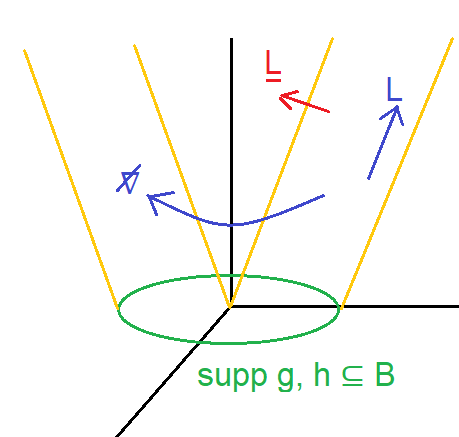
\includegraphics[scale = 0.5]{peeling}
\end{center}
Recall the radial derivative is given by $\partial_r := \frac1r \sum_j x^j \partial_j$. Define the derivatives $L$ in the $t + r$ direction, $\underline L$ in the $t - r$ direction, and $\slashed \nabla$ in the rotational direction. More concretely, 
\begin{align*}
	L
		:= \partial_t + \partial_r, \qquad
	\underline L
		:= \partial_t - \partial_r, \qquad
	\slashed\nabla_j  
		:= \partial_j  - \frac{x^j}{r} \partial_r  = \sum_{k = 1}^d \frac{x^j}{r^2} \Omega_{j, k} .
\end{align*}		
We aim to show that the ``good'' derivatives $\overline \partial \in \{ L, \slashed \nabla \}$ improve decay by $t$ in comparison to decay of the total derivative $\partial$ in Corollary \ref{cor:totaldisp}. 

\begin{theorem}[``Peeling'' for ``good" derivatives]
	Let $\phi \in C^1 (\R_t \times \R^d_x)$, then 
		\[ |\overline \partial \phi (t, x) | \lesssim \frac{1}{1 + t + r} \sum_{|\alpha| = 1} |Z^\alpha \phi (t, x)|.\] \label{thm:peel}
\end{theorem}

\begin{proof}
	We first note the case $t + r \leq 1$ is trivial since the right-hand side controls all first-order derivatives. Suppose then $t + r > 1$, and note
		\begin{align*}
			\frac{1}{t + r} \left( S + \sum_{j = 1}^d \frac{x^j}{r} H_j \right) 
				&= \frac{1}{t + r} \left( t \partial_t + \sum_{j = 1}^d x^j \partial_j + \sum_{j = 1}^d \frac{x^j}{r} \left( t \partial_j + x^j \partial_t \right) \right)\\
				&= \frac{1}{t + r} \left( (t + r)\partial_t + \sum_{j = 1}^d \frac{x^j (t + r)}{r} \partial_j\right)  = \partial_t + \partial_r = L.
		\end{align*}
	This proves the result for $\overline\partial = L$. For the rotational derivative, note the identity
		\begin{align*}
			\frac1t \left( x^j H_k - x^k H_j\right)
				&= \frac1t \left( x^j t \partial_k + x^j x^k \partial_t -  x^k t \partial_j -x^j x^k \partial_t  \right) = \Omega_{j, k}.
		\end{align*}	
	It follows from the identity above and the definition of $\slashed \nabla$ that 
		\[ |\slashed \nabla \phi| \lesssim \frac1r \sum_{j, k = 1}^d |\Omega_{j, k} \phi| \lesssim \frac1t \sum_{j = 1}^d |H_j \phi|. \]
	This proves the result for $\overline\partial =\slashed \nabla$.	
\end{proof}

\begin{corollary}
	Let $\phi$ be a solution to the $(1 + d)$-dimensional linear homogeneous wave equation (\ref{eq:linearwave}) with initial data $g, h \in C^\infty_c (B(0, R))$. Then 
		\[ |\overline \partial \phi (t, x)| \lesssim_{d, R} \frac{(1 + |t - r|)^\frac12}{(1 + t + r)^{\frac{d + 1}{2}}} \sum_{|\alpha| \leq \lfloor \frac{d + 4}{2} \rfloor} ||\partial Z^\alpha \phi ||_{L^2_x} (0). \]
\end{corollary}

\begin{proof}
	Since $Z^\alpha \phi$ also solve the linear homogeneous wave equation with initial data $Z^\alpha g, Z^\alpha h \in C^\infty_c (B(0, R))$, it follows from Corollary \ref{cor:goodlemma} that
		\[   \sum_{|\alpha| = 1} |Z^\alpha \phi (t, x)| \lesssim_{d, R}  \frac{(1 + |t - r|)^{\frac12}}{(1 + t + r)^{\frac{d - 1}{2}} } \sum_{|\alpha| \leq \lfloor \frac{d + 4}{2} \rfloor} ||\partial Z^\alpha \phi ||_{L^2_x} (0). \]
	Combining with the peeling property and rearranging finishes the proof.
\end{proof}

\begin{remark}
	Note in four-dimensional space-time $\R_t \times \R^3_x$ we only have the estimate $||\partial \phi||_{L^\infty_x} (t) \lesssim 1/t$, which is not integrable in time, however our estimate for the ``good'' derivatives $||\overline\partial \phi||_{L^\infty_x} (t) \lesssim 1/t^{3/2}$ is integrable in time.  
\end{remark}

Generally, we will not have symmetry in the quadratic non-linearity as we did when considering the equation $\Box \phi = \partial \phi \partial \phi$. Consequently, it will not be enough to place the ``good'' derivatives in $L^\infty_x$; we will also need a weighted $L^2_{t, x}$-estimate.

\begin{theorem}[Energy estimate on null cones]
	Let $\phi$ be a solution to the inhomogeneous wave equation $\Box \phi = f$ for smooth compactly supported initial data, then for $\delta > 0$,
		\[ || \nabla_{t, x} \phi ||_{L^\infty_t L^2_x (0, T)} + ||(1 + |t - r|)^{-\frac12 - \delta} \, \overline\partial \phi||_{L^2_{t, x}(0, T)} \lesssim_\delta ||\nabla_{t, x} \phi||_{L^2_x} (0) + ||f||_{L^1_t L^2_x (0, T)} . \]
		\label{thm:nullenergy}
\end{theorem}

\begin{proof}
	By the usual energy estimate, Corollary \ref{cor:energyest1}, it suffices to control the weighted $L^2$-norm of the ``good'' derivative. Recall from the proof of conservation of energy, Theorem \ref{thm:conserve}, that we can write $f \partial_t \phi$ as a divergence, 
				\begin{align*}
		f \partial_t \phi 
			&= \partial_t \left( -\frac12 (\partial_t \phi)^2 - \frac12 \sum_{j = 1}^n (\partial_j \phi)^2 \right) + \nabla_x \cdot (\partial_t \phi \, \nabla_x \phi) = \nabla_{t, x} \cdot \left( -\frac12 |\nabla_{t, x} \phi|^2, \partial_t \phi \nabla_x \phi \right).
	\end{align*}
	However, rather than integrating on $[0, T] \times \R^d_x$, we instead integrate on the null cones 
		\[C_{u_0} = \{ (t, x) :  u + u_0 = 0 \text{ and } t \in [0, T] \}, \qquad u := t - r. \]
	By a change of coordinates and $L^2_u$-integrability of $(1 + |u|)^{-\frac12 - \delta}$, we can write
		\[ ||(1 + |u|)^{-\frac12 - \delta}\, \overline\partial \phi||_{L^2_{t, x} (0, T)} \sim || (1 + |u|)^{-\frac12 - \delta}  \overline\partial \phi||_{L^2_u L^2 (C_u)} \lesssim \sup_{u} ||\overline \partial \phi ||_{L^2 (C_u)}.\]	
	It remains to control the right-hand side above. We argue as we did in the usual energy estimate, however we instead integrate over the cone region $R \subseteq [0, T] \times \R^n_x$ with boundary $\partial R = C_u + B_1 + B_2$,
	\begin{center}
		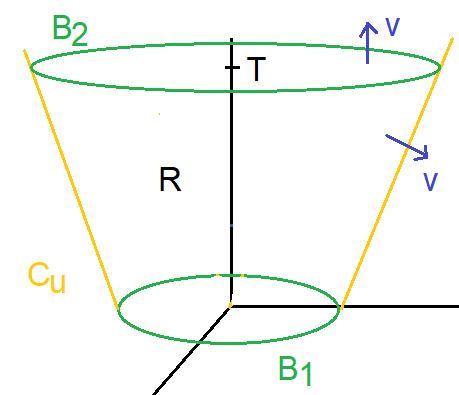
\includegraphics[scale = 0.5]{divergence}
	\end{center}
	and applying the divergence theorem gives
		\begin{align*}
			\int_R f \partial_t \phi \, dA
				& = \int_{C_{u} + B_1 + B_2} \left( -\frac12 |\nabla_{t, x} \phi|^2, \partial_t \phi \nabla_x \phi \right) \cdot \nu \, dS \\
				&= \int_{C_{u}} \left( -\frac12 |\nabla_{t, x} \phi|^2, \partial_t \phi \nabla_x \phi \right) \cdot  \left( \frac12, -\frac{x}{2|x|} \right)  dS + \frac12 || \nabla_{t, x} \phi||^2_{L^2_x (|x| \leq u)} (0) - \frac12 ||\nabla_{t, x} \phi||_{L^2_x (|x| \leq u + T)}^2 (T).
		\end{align*}	
	Observe that the integral on the null cone $C_u$ takes the form
		\begin{align*}
			\int_{C_u} \left( -\frac12 |\nabla_{t, x} \phi|^2, \partial_t \phi \nabla_x \phi \right) \cdot \left( 1, -\frac{x}{|x|} \right) dS
				&= - \frac12 \int_{C_u} \left( |\nabla_{t, x} \phi|^2  + 2 \sum_{i = 1}^n \frac{x_i}{|x|} \partial_t \phi \partial_i \phi \right) dS \\
				&= - \frac12 \int_{C_u} \left( (\partial_t \phi)^2 + (\partial_r \phi)^2 + |\slashed \nabla \phi|^2 + 2\partial_t \phi \partial_r \phi\right) dS\\
				&= - \frac12 \int_{C_u} \left(|\slashed \nabla \phi|^2 + |(\partial_t + \partial_r) \phi|^2\right)  dS\\
				&= -\frac12 \int_{C_u} \left(|\slashed \nabla \phi|^2 + |L \phi|^2 \right)  dS = - \frac12 \int_{C_u} |\overline\partial \phi|^2 dS = ||\overline \partial \phi||_{L^2 (C_u)}^2.
		\end{align*}	
	Rearranging, we conclude
			\[  \sup_{u} ||\overline \partial \phi ||_{L^2 (C_u)} \lesssim || \nabla_{t, x} \phi ||_{L^\infty_t L^2_x (0, T)}  +  ||\nabla_{t, x} \phi||_{L^2_x} (0)+ ||f||_{L^1_t L^2_x (0, T)}.\]
	This completes the proof. 	
\end{proof}

\subsection{The null condition}

\begin{definition}
	Given a matrix $Q \in \R^{d \times d}$, we say that $Q(\phi, \psi) := \sum_{j, k} Q^{j, k} \partial_j \phi \partial_k \psi$ is a \emph{null form} if it satisfies the \emph{null condition}: $\sum_{j, k} Q^{i, j} \xi_j \xi_k = 0$ whenever $\sum_{j, k} M^{j, k} \xi_j \xi_k = 0$.
\end{definition}

\begin{lemma}[Properties of null forms]
	Let $Q \in \R^{3 \times 3}$ be a null form, then the following properties hold:
	\begin{enumerate}
		\item The space of null forms is linearly generated by the Minkowski metric $M$ and the anti-symmetric matrices. 
	
		\item The null form is controlled by
					\[ |Q( \phi,  \psi)| \lesssim |\partial \phi| |\overline\partial \psi| + |\overline\partial \phi| |\partial \psi|.\]
		\item Given a commuting vector field $Z \in \{ \partial_t, \partial_j, \Omega_{jk}, H_j,  S \}$, we have
						\[ Z(Q( \phi,\psi)) = Q(Z\phi, \psi) + Q(\phi, Z \psi) + \tilde Q(\phi, \psi) \]
					for some null form $\tilde Q$. 	
	\end{enumerate}
\end{lemma}

\begin{proof}
\leavevmode
\begin{enumerate}
	\item The Minkowski metric $M$ trivially satisfies the null condition. Suppose $B^\top = - B$, then $\xi^\top B \xi = - \xi^\top B \xi$, which holds if and only if $\xi^\top B \xi = 0$. Hence, anti-symmetric matrices also trivially satisfy the null condition. Conversely, $Q$ can be written as the sum of symmetric and anti-symmetric matrices, namely
				\[ Q = \frac{Q + Q^\top}{2} + \frac{Q - Q^\top}{2} =: A + B. \]
			Then
				\[ 0 =  \xi^\top Q \xi = \xi^\top A \xi + \xi^\top B \xi = \xi^\top A \xi\]
	whenever $\xi^\top M \xi = 0$. Since $A$ is symmetric, $\xi^\top A \xi$ is a homogeneous polynomial in $\xi$ of degree $2$ which has a zero set coinciding with that of $\xi_0^2 - \sum_j \xi_j^2$. This holds if and only if $A$ is a constant multiple of $M$. 

	\item By a., it suffices to check the result for the Minkowski metric $M$ and anti-symmetric null forms $B$. The former case follows from the identity
					\[ M(\phi, \psi) = \sum_{j, k = 1}^3 M^{j, k} \partial_j \phi \partial_k \psi = \partial_t \phi \partial_t \psi - \sum_{j = 1}^3 \partial_j \phi \partial_j \psi = 2L \phi \underline L \psi + 2 \underline L \phi L \psi - \slashed \nabla \phi \cdot \slashed \nabla \psi. \]
				Each term on the right contains at least a factor of one ``good'' derivative, so the desired bound holds. 
	\item By a., it suffices to check the result for the Minkowski metric $M$ and anti-symmetric null forms $B$. This is an exercise in linear algebra and calculus. 
\end{enumerate}f\
\end{proof}

\begin{remark}
	b. guarantees that each term in the quadratic non-linearity from a null form contains at least one ``good'' derivative $\overline \partial$. By the peeling property, $|\overline \partial \phi|$ decays better than $|\partial \phi|$, and moreover the decay is integrable in time. Hence we put one of the of the two factors in the quadratic term in $L^2$ and the other in $L^\infty$. 
	
	c. guarantees that the null structure is preserved after differentiating by a commuting vector field $Z$. This allows us to extend our energy estimates on $\phi$ to $Z \phi$. 
\end{remark}

\begin{theorem}[Null structure energy estimate]
	Let $\phi$ be a solution to 
		\begin{equation}
			\Box \phi = Q(\phi, \phi) \label{eq:nullwave}
		\end{equation}
	on $\R_t \times \R^3_x$ with smooth compactly supported initial data. There exists $\epsilon > 0$ such that if
		\[ \sum_{|\alpha| \leq 5} ||\nabla_{t, x} Z^\alpha \phi||_{L^2_x} (0) \leq \epsilon \]
	then 		
		\[   \sum_{|\alpha| \leq 5} ||\nabla_{t, x} Z^\alpha \phi||_{L^2_x} (t) \lesssim   \sum_{|\alpha| \leq 5} ||\nabla_{t, x} Z^\alpha \phi||_{L^2_x} (0). \]
\end{theorem}

\begin{proof}
	We can write
		\[ \sum_{|\alpha| \leq 5} | \Box Z^\alpha \phi| \lesssim \sum_{|\beta| + |\gamma| \leq 5} |\overline \partial Z^\beta \phi| |\partial Z^\gamma \phi| \leq \left(\sum_{|\beta| \leq 2} |\overline \partial Z^\beta \phi| \right)\left( \sum_{|\gamma| \leq 5} |\partial Z^\gamma \phi| \right) + \sum_{|\beta| \leq 5, \, |\gamma| \leq 2} |\overline \partial Z^\beta \phi \partial Z^\gamma \phi|, \]
	where the first inequality holds since the commuting vector fields preserve the null structure. For the first term on the right, we put $\overline \partial$ in $L^\infty_x$ and apply Theorem \ref{thm:peel} the peeling property, and the Klainerman-Sobolev inequality, and we place $\partial$ into $L^2_x$, which gives us
		\[\left|\left| \left(\sum_{|\beta| \leq 2} |\overline \partial Z^\beta \phi| \right)\left( \sum_{|\gamma| \leq 5} |\partial Z^\gamma \phi| \right) \right|\right|_{L^1_t L^2_x(0, T)}\lesssim \int_0^T \frac{1}{(1 + t)^{\frac32}} \left( \sum_{|\alpha| \leq 5} || \partial Z^\alpha \phi ||_{L^2_x} \right)^2 dt \leq 2  \left( \sum_{|\alpha| \leq 5} || \partial Z^\alpha \phi ||_{L^\infty_t L^2_x (0, T)} \right)^2  \]
	For the second term, we apply Cauchy-Schwartz in $t$ to put $\overline\partial$ into weighted $L^2_{t, x}$ and $\partial$ into weighted $L^2_t L^\infty_{x}$,
		\begin{align*}
			\sum_{|\beta| \leq 5, \, |\gamma| \leq 2}  ||\overline \partial Z^\beta \phi \partial Z^\gamma \phi ||_{L^1_t L^2_x (0, T)} 
				&\leq \left(\sum_{|\beta| \leq 5}  || (1 + |t - r|)^{-\frac{1 + \delta}{2}} \overline \partial Z^{\beta} \phi ||_{L^2_{t, x} (0, T)}\right) \left(\sum_{|\gamma| \leq 2} || (1 + |t - r|)^{\frac{1 + \delta}{2}} \partial Z^\gamma \phi ||_{L^2_t L^\infty_x (0, T)} \right).
		\end{align*}
	For the weighted $L^2_t L^\infty_{x}$ term above, we apply Klainerman-Sobolev,
		\[ \left(\sum_{|\gamma| \leq 2} || (1 + |t - r|)^{\frac{1 + \delta}{2}} \partial Z^\gamma \phi ||_{L^2_t L^\infty_x (0, T)} \right) \lesssim \int_0^T \frac{1}{(1 + t)^{2-\delta}} \sum_{|\alpha| \leq 5} ||\partial Z^\alpha \phi||_{L^2_x} dt \lesssim_\delta \sum_{|\alpha| \leq 5} ||\partial Z^\alpha \phi||_{L^\infty_t L^2_x (0, T)}  \]
	where the last inequality follows from integrability of $1/(1 + t)^{2 - \delta}$ for $0 < \delta < 1$. Collecting our results, it follows from Theorem \ref{thm:nullenergy} the energy estimate on the null cone, applied to $Z^\alpha \phi$ that 
		\begin{align*}
			\sum_{|\alpha| \leq 5} ||\nabla_{t, x} Z^\alpha \phi ||_{L^2_x} 
				&+ ||(1 + |t - r|)^{-\frac{1 + \delta}{2}} \overline\partial Z^\alpha \phi||_{L^2_{t, x}} \\
				&\leq C\sum_{|\alpha| \leq 5} ||\nabla_{t, x} Z^\alpha \phi||_{L^2_x} (0) +C \left( \sum_{|\alpha| \leq 5} || \nabla_{t, x} Z^\alpha \phi ||_{L^\infty_t L^2_x (0, T)} \right)^2 \\
				&\qquad + C \left(\sum_{|\alpha| \leq 5}  || (1 + |t - r|)^{-\frac{1 + \delta}{2}} \overline \partial Z^{\alpha} \phi ||_{L^2_{t, x} (0, T)}\right) \left(\sum_{|\alpha| \leq 5} ||\nabla_{t, x} Z^\alpha \phi||_{L^\infty_t L^2_x (0, T)}  \right)
		\end{align*}	
	for some implicit constant $C > 0$ depending only on $k = 5$ and $0 < \delta < 1$. We conclude the result by a bootstrap argument; let $B \geq 2 (C + 1)$ and suppose $T \geq 0$ such that	
		\[ \sum_{|\alpha| \leq 5} ||\nabla_{t, x} Z^\alpha \phi ||_{L^\infty_t L^2_x (0, T)} +  ||(1 + |t - r|)^{-\frac{1 + \delta}{2}} \, \overline\partial Z^\alpha \phi||_{L^2_{t, x}(0, T)} \leq  B\sum_{|\alpha| \leq 5} ||\nabla_{t, x} Z^\alpha \phi||_{L^2_x} (0). \]
	The result clearly holds for $T  = 0$ by choice of $B \geq 1$, so the base case of our continuous induction on time is satisfied. We aim to prove a stronger bound than the one assumed. The previous two inequalities imply 
		\begin{align*}
			\sum_{|\alpha| \leq 5} ||\nabla_{t, x} Z^\alpha \phi ||_{L^2_x} (t)  + ||(1 + |t - r|)^{-\frac{1 + \delta}{2}} \overline\partial Z^\alpha \phi||_{L^2_{t, x}}
				&\leq C\sum_{|\alpha| \leq 5} ||\nabla_{t, x} Z^\alpha \phi||_{L^2_x} (0) +C B^2 \left( \sum_{|\alpha| \leq 5} || \nabla_{t, x}Z^\alpha \phi ||_{L^2_x} (0) \right)^2.
		\end{align*}	
	To complete the argument, it suffices to show the right-hand side satisfies the bound
		\[ C\sum_{|\alpha| \leq 5} ||\nabla_{t, x} Z^\alpha \phi||_{L^2_x} (0) +C B^2 \left( \sum_{|\alpha| \leq 5} || \nabla_{t, x} Z^\alpha \phi ||_{L^2_x} (0) \right)^2 \leq \frac12 B \sum_{|\alpha| \leq 5} ||\nabla_{t, x} Z^\alpha \phi||_{L^2_x} (0). \]
	Rearranging, it is equivalent to show
		\[ CB^2 \sum_{|\alpha| \leq 5} ||\nabla_{t, x} Z^\alpha \phi||_{L^2_x} (0) \leq \frac12 B - C. \]
	Given data sufficiently small, i.e. $\epsilon \ll 1$, completes the proof. 			
\end{proof}


\section{Einstein vacuum equation}
\input{einstein}

\bibliography{biblio}
\bibliographystyle{alpha} 

\end{document}